% chose the documnet class as article
\documentclass{article}

% basic setteings
\topmargin=-0.45in
\evensidemargin=0in
\oddsidemargin=0in
\textwidth=6.5in
\textheight=9.0in
\headsep=0.25in

% create a new command 
\newcommand{\hwtitle}{Network Measures: Homework\ \#2}
\newcommand{\student}{Zeng Xiangrong}
\newcommand{\teacher}{Professor Hao Wang}

% this package is used for setting header and footer
\usepackage{fancyhdr}
\pagestyle{fancy}
\usepackage{graphicx}

\begin{document}
% set the title page
\begin{titlepage}
\begin{center}
    \textbf{}
    \\[4.5cm]
    \textbf{\huge \hwtitle}
    \\[0.3cm]
    \textnormal{Due on}
    \today
    \\[0.4cm]
    \emph{\teacher}
    \\[8cm]
    \textbf{\Large \student}
\end{center}
\end{titlepage}

% setting the header and footer
\fancyhf{} % clear the header and footer
\lhead{\student}
\chead{\hwtitle}
\rhead{problem \thesection}
\renewcommand{\footrulewidth}{0.4pt}
\cfoot{\thepage}

% setting the section style
\setcounter{section}{0} % set the counter start from 0
% set the section style to "problem 1" and increase correctly
\renewcommand{\section}{
    \stepcounter{section}
    \begin{flushleft}
        \raggedright \Large\textbf{Problem \thesection\\}
    \end{flushleft}}

% main contex
\section
% put the main text of every problem here
    Given graph(fig.1), 
    compute the three central nodes based on \emph{degree, eigenvector,
    Katz($\alpha=\beta=0.3$), PageRank, betweenness and closeness}
    centrality methods.
    You should implement all these centrality methods by c, c++, java or c\#
    \\
    \begin{figure}[h]
        \center
        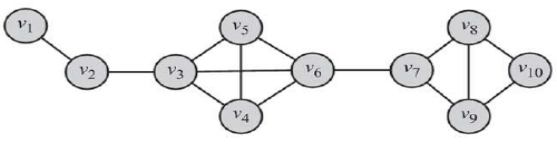
\includegraphics[width = 0.8\linewidth]{hw2.jpg}
        \caption{Graph}
    \end{figure}
\subsection*{Solution}
\begin{table}[h]
        \caption{Results}
        \begin{center}
            \begin{tabular}{llll}
                \hline
                & First node& Second node& Thrid node\\
                \hline
                degree centrality&1&2&4\\
                eigenvector centrality&0.05&0.16&0.47\\
                Katz centrality&1.57&4.24&11.56\\
                Pagerank centrality&0.37&0.45&0.48\\
                betweenness centrality&0&16&28\\
                closeness centrality&0.28&0.38&0.5\\
                \hline
            \end{tabular}
        \end{center}
    \end{table}


\clearpage % end current page

\end{document}
